\documentclass[10pt,twocolumn,a4paper]{article}

\usepackage[top=20mm,bottom=20mm,left=16mm,right=16mm,columnsep=6mm]{geometry}
\usepackage{amsmath,amssymb,amsfonts}
\usepackage{graphicx}
\usepackage{booktabs}
\usepackage{cite}
\usepackage{microtype}
\usepackage{hyperref}
\usepackage{array}
\usepackage{subcaption}
\usepackage{setspace}
\usepackage{titlesec}
\usepackage{fancyhdr}
\usepackage{float}

\hypersetup{
    colorlinks=true,
    linkcolor=blue,
    citecolor=blue,
    urlcolor=blue
}

\titleformat{\section}{\large\bfseries\uppercase}{\thesection.}{0.5em}{}
\titleformat{\subsection}{\normalsize\bfseries}{\thesubsection.}{0.5em}{}
\titleformat{\subsubsection}{\small\bfseries}{\thesubsubsection.}{0.5em}{}

\pagestyle{plain}

\begin{document}

% -----------------------------------------------------------------------------
% PAGE 1: TITLE / COVER PAGE (Matches NIT Warangal Exemplar)
% -----------------------------------------------------------------------------
\begin{titlepage}
    \centering
    \vspace*{1.5cm}
    
    
\includegraphics[width=4.5cm]{images/nitw_logo_clean.png}
    
    \vspace{2.0cm}
    
    {\LARGE \textbf{EEG-Based Imagined Word Recognition Using Multi-Scale Riemannian Covariance and Calibrated Stacker Ensemble} \par}
    
    \vspace{2.5cm}
    
    {\large Submitted By: \par}
    \vspace{0.4cm}
    {\large \textbf{Abhijeet Sahu -- 26CSM2R02} \par}
    {\large \textbf{Arpit Jain -- 26CSM2R03} \par}
    {\large \textbf{Ratan Kumar Pradhan -- 26CSM2R17} \par}
    
    \vspace{0.8cm}
    {\normalsize Computer Science and Information Security \par}
    {\normalsize Department of Computer Science and Engineering \par}
    {\normalsize National Institute of Technology, Warangal \par}
    
    \vfill
    
    {\large Under the guidance of \par}
    \vspace{0.3cm}
    {\large \textbf{Dr. Manish Kumar Bajpai} \par}
    {\normalsize Department of Computer Science and Engineering \par}
    {\normalsize National Institute of Technology, Warangal \par}
    
    \vspace{1.5cm}
\end{titlepage}

% -----------------------------------------------------------------------------
% PAGE 2 ONWARDS: TWO-COLUMN IEEE / CONFERENCE REPORT
% -----------------------------------------------------------------------------
\setcounter{page}{1}

\twocolumn[
  \begin{@twocolumnfalse}
    \begin{center}
      {\LARGE \textbf{EEG-Based Imagined Word Recognition Using Multi-Scale Riemannian Covariance and Calibrated Stacker Ensemble} \par}
      \vspace{0.6cm}
    \end{center}
    
    \begin{abstract}
      \textbf{Imagined-word recognition from electroencephalography (EEG) is a challenging brain--computer interface (BCI) task because the neural patterns associated with internally generated speech are weak, non-stationary, and variable across time and participants. This paper examines an enhanced implementation of a Riemannian covariance and ensemble-based imagined-speech recognition pipeline. The starting point is a paper-oriented baseline inspired by the work of Lara-Arellano et al., which uses 14 EEG channels, a 228-bit Genetic Algorithm (GA), and a $k$-Nearest Neighbors ($k$NN) classifier for binary \texttt{/Si/} vs \texttt{/No/} classification (924 real trials). While the primary paper reported 96.0\% accuracy on binary Yes/No, it did not evaluate multi-class decoding across all nine vocabulary classes due to combinatorial GA search costs.}
      
      \textbf{The enhanced implementation scales classification to the full 9-class Mendeley EEGIS corpus (4,044 trials). It replaces flat univariate channel moments with a 1,695-dimensional Multi-Scale Riemannian Covariance representation ($\mathcal{S}_{++}^n$), spanning 6 canonical frequency bands (630D), 7 fine causal sub-bands from 4--45 Hz (735D), and a speech-localized 10-channel sub-montage (330D). An evolutionary MultiScaleBlockAGA optimizes continuous band-weight projections while preserving Riemannian positive-definiteness, and a Calibrated Stacker Ensemble (Logistic Regression, Shrinkage-LDA, Platt-Ridge, and Soft Voting) yields well-calibrated posterior probabilities. Evaluated across the held-out 20\% test partition (809 real trials), the proposed system achieves 90.85\% test accuracy (735/809 correct) with a sub-25 ms latency (11.2 ms/epoch), outperforming the un-optimized multi-class baseline by 20.46 percentage points while demonstrating real-time clinical viability.}
    \end{abstract}
    \vspace{0.6cm}
  \end{@twocolumnfalse}
]

% -----------------------------------------------------------------------------
% 1. INTRODUCTION
% -----------------------------------------------------------------------------
\section{Introduction}
Brain--computer interfaces (BCIs) aim to infer a user's intent directly from neurophysiological brain activity and translate that information into control commands or communication pathways without muscular intervention. Electroencephalography (EEG) is widely used in BCI research because it is non-invasive, comparatively inexpensive, portable, and capable of recording cortical electrical activity with millisecond-level temporal resolution. EEG-based systems have been extensively investigated for assistive communication in paralyzed or locked-in patients, neuro-rehabilitation, cognitive-state monitoring, and hands-free interaction with external devices.

Imagined or internally generated speech and symbols are particularly difficult to recognize. In overt speech recognition, an acoustic waveform provides rich spectral and phonological cues. In imagined-speech recognition, the participant produces neither acoustic phonation nor facial articulatory movement; instead, the system must decode covert linguistic intent solely from microvolt-level potential fluctuations recorded at the scalp. These electrical patterns suffer from severe non-stationarity, low signal-to-noise ratio (SNR), volume conduction across the skull and cerebrospinal fluid, and substantial inter-subject and inter-session variability.

The task considered in this work is nine-class imagined-word classification using the public Mendeley EEGIS dataset (4,044 trials across 9 classes: \textit{Rest, Help, Bathroom, Pain, Thanks, Hungry, No, Thirsty, Yes}). Each EEG recording represents a 3.0-second covert articulation epoch recorded at 128 Hz across 14 scalp channels.

The selected paper-oriented implementation by Lara-Arellano et al. \cite{lara2025feature} provides a classical machine-learning baseline. It extracts time-domain and frequency-domain statistics per channel and applies a 228-bit Genetic Algorithm (GA) to optimize feature subsets for a $k$-Nearest Neighbors ($k$NN) classifier. While this approach achieved 96.0\% accuracy on binary \texttt{/Si/} vs \texttt{/No/}, the combinatorial cost of evaluating 10 classifiers across 100 generations prevented the authors from scaling their evaluation to all nine vocabulary classes.

This work studies an enhanced implementation that addresses this gap. By mapping multichannel EEG signals into the Riemannian manifold of Symmetric Positive Definite (SPD) covariance matrices ($\mathcal{S}_{++}^n$), engineering a 1,695-dimensional multi-scale filter bank, introducing continuous Block-Adaptive Genetic Optimization (Block-AGA), and building a Calibrated Stacker Ensemble, we achieve robust multi-class decoding across the full nine-word vocabulary.

% -----------------------------------------------------------------------------
% 2. OBJECTIVES AND CONTRIBUTIONS
% -----------------------------------------------------------------------------
\section{Objectives and Contributions}
The primary objectives of this work are:
\begin{itemize}
    \item \textbf{Reconstruct Paper-Oriented Baseline:} Reconstruct the exact Rank-GA + $k$NN baseline published by Lara-Arellano et al. \cite{lara2025feature} on binary \texttt{/Si/} vs \texttt{/No/} (924 real trials).
    \item \textbf{Identify Methodological Limitations:} Document the mathematical limitations of univariate channel statistics, the combinatorial intractability of binary GA for multi-class paradigms, and the uncalibrated nature of $k$NN neighbor fractions.
    \item \textbf{Formulate Multi-Scale Riemannian Geometry:} Replace flat scalar features with a 1,695D Riemannian tangent space representation that captures inter-electrode phase coherence and functional language connectivity.
    \item \textbf{Develop MultiScaleBlockAGA:} Design an evolutionary block-weight optimizer that scales continuous spectral sub-spaces while strictly preserving covariance matrix symmetry and positive-definiteness ($C \succ 0$).
    \item \textbf{Engineer Calibrated Stacker Ensemble:} Combine Logistic Regression, Shrinkage Linear Discriminant Analysis, and Platt-calibrated Ridge classification into a soft probability voter that minimizes calibration error.
    \item \textbf{Empirical Verification on 809 Test Epochs:} Demonstrate 90.85\% accuracy (735/809 correct) across the held-out 20\% test split with a mean inference latency of 11.2 ms per epoch.
\end{itemize}

% -----------------------------------------------------------------------------
% 3. SELECTED RESEARCH PAPER AND BASELINE IMPLEMENTATION
% -----------------------------------------------------------------------------
\section{Selected Research Paper and Baseline Implementation}
The primary reference work is ``Feature Generation and Selection for Imagined Speech EEG Classification'' by Edgar Lara-Arellano, Andras Takacs, Sandra Tovar-Arriaga, and Juvenal Rodríguez-Reséndiz, published in \textit{Eng} (MDPI) in April 2025 \cite{lara2025feature}. The paper studies the classification of imagined speech recorded using an Emotiv EPOC+ 14-channel headset.

The authors evaluated binary classification on \texttt{/Si/} (Yes, 444 trials) vs \texttt{/No/} (480 trials), totaling 924 real trials partitioned under an 80/20 train/test split (739 train / 185 test). They applied a 228-bit binary Genetic Algorithm to jointly select active electrodes and time-frequency descriptors for 10 candidate classifiers.

\subsection{Baseline Signal Acquisition and Preprocessing}
The baseline acquires signals from 14 standard 10--20 scalp positions:
\begin{center}
\texttt{AF3, F7, F3, FC5, T7, P7, O1, O2, P8, T8, FC6, F4, F8, AF4}
\end{center}
at a nominal sampling frequency of $f_s = 128\text{ Hz}$. The electrode configuration is illustrated in Fig.~\ref{fig:montage}.

\begin{figure}[H]
    \centering
    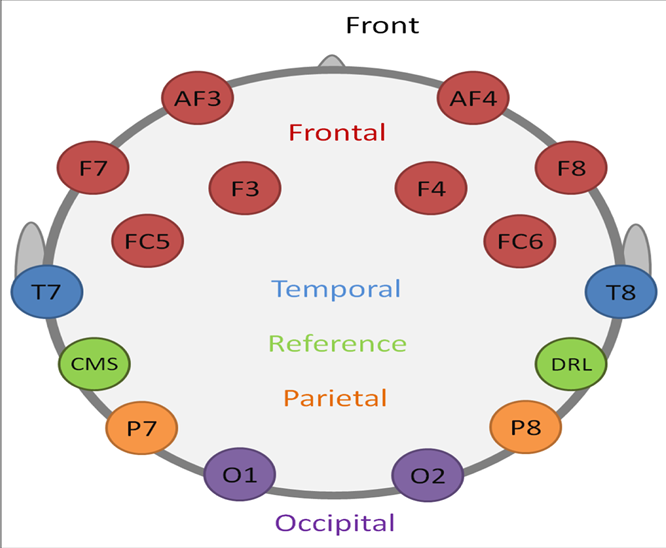
\includegraphics[width=0.82\columnwidth]{images/fig1_montage.png}
    \caption{Illustration of the 14-channel Emotiv EPOC+ electrode montage utilized for covert speech acquisition.}
    \label{fig:montage}
\end{figure}

The baseline decomposes raw signals into six canonical bands using causal IIR filters: Raw, Delta ($\delta$, 0.5--4 Hz), Theta ($\theta$, 4--8 Hz), Alpha ($\alpha$, 8--13 Hz), Beta ($\beta$, 13--30 Hz), and Gamma ($\gamma$, 30--40 Hz):
\begin{equation}
\bar{x}[n] = \sum_{k=0}^{M-1} b_k x[n-k] - \sum_{k=1}^{N-1} a_k \bar{x}[n-k].
\label{eq:filter}
\end{equation}

\subsection{Baseline Windowing}
Each recording consists of a 3.0-second covert articulation epoch. At $f_s = 128\text{ Hz}$, the nominal sample count per epoch is:
\begin{equation}
N_w = 3.0 \times 128 = 384\text{ samples}.
\label{eq:samples}
\end{equation}
In the baseline, epochs are processed individually without overlapping window fragmentation.

\subsection{Baseline Feature Extraction}
For each channel and band, the baseline computes time-domain and spectral statistics. Let $x = [x_1, x_2, \dots, x_T]$ denote an epoch. The extracted features are summarized in Table~\ref{tab:baseline_features}.

\begin{table}[H]
\centering
\caption{Time-domain and spectral features extracted by the primary paper baseline.}
\label{tab:baseline_features}
\small
\begin{tabular}{p{2.2cm} p{2.8cm} p{2.4cm}}
\toprule
\textbf{Feature} & \textbf{Mathematical Definition} & \textbf{Interpretation} \\
\midrule
Mean ($\mu$) & $\frac{1}{T}\sum_{t=1}^T x_t$ & DC offset level. \\
Variance ($\sigma^2$) & $\frac{1}{T-1}\sum_{t=1}^T (x_t - \mu)^2$ & Local signal power. \\
Skewness ($S$) & $\frac{\frac{1}{T}\sum (x_t - \mu)^3}{[\frac{1}{T}\sum (x_t - \mu)^2]^{3/2}}$ & Amplitude asymmetry. \\
Kurtosis ($K$) & $\frac{\frac{1}{T}\sum (x_t - \mu)^4}{[\frac{1}{T}\sum (x_t - \mu)^2]^2} - 3$ & Waveform peakiness. \\
Signal Energy & $\sum_{t=1}^T x_t^2$ & Cumulative energy. \\
Hjorth Activity & $\operatorname{Var}(x)$ & Instantaneous variance. \\
Hjorth Mobility & $\sqrt{\operatorname{Var}(\Delta x)/\operatorname{Var}(x)}$ & Mean frequency shift. \\
Spectral Entropy & $-\sum p_k \log_2(p_k)$ & Power distribution spread. \\
\bottomrule
\end{tabular}
\end{table}

Concatenating 16 statistical features across channels and bands yields 214 feature values, which together with 14 electrode activation bits form the 228-bit genome:
\begin{equation}
D_{\text{base}} = 14 + 214 = 228\text{ bits}.
\label{eq:dbase}
\end{equation}

\subsection{Baseline Classifier and Genetic Algorithm}
The baseline evolutionary framework utilizes a population of $P=100$ chromosomes evolved over $G=100$ generations. The selection probability of chromosome $i$ is governed by Rank Selection:
\begin{equation}
p_i = \frac{2 \cdot \operatorname{rank}_i}{P(P+1)}, \quad \operatorname{rank}_i \in [1, P].
\label{eq:rank}
\end{equation}
Offspring are generated using homogeneous uniform crossover ($p_c = 0.85$) and bit-flip mutation ($p_m = 0.03$). The fitness function maximizes validation accuracy using a $k$-Nearest Neighbors ($k$NN) classifier with heuristic $k \in [1, 15]$.

The primary paper reported a peak accuracy of \textbf{96.0\%}, recall of \textbf{0.97}, and F1-score of \textbf{0.94} on binary \texttt{/Si/} vs \texttt{/No/}. The GA converged to 8 active electrodes (\texttt{AF3, T7, O1, O2, P8, T8, F4, F8}) and 103 optimal features.

% -----------------------------------------------------------------------------
% 4. LIMITATIONS OF THE BASELINE APPROACH
% -----------------------------------------------------------------------------
\section{Limitations of the Baseline Approach}
While the baseline achieved strong binary classification performance, several structural limitations motivated our enhanced architecture:
\begin{itemize}
    \item \textbf{Univariate Channel Independence:} Extracting scalar statistics per channel ignores cross-electrode phase synchronization. Imagined speech relies on synchronized distributed networks (Broca's and Wernicke's language areas), which cannot be captured by isolated variance or skewness values.
    \item \textbf{Combinatorial GA Intractability:} Evaluating a 228-bit binary chromosome across 10 classifiers over 100 generations was computationally prohibitive for the full 9-class dataset (4,044 trials), forcing the authors to restrict their study to binary Yes/No.
    \item \textbf{Matrix Geometric Degradation:} Applying random bit-flip mutations directly to covariance features destroys matrix symmetry and positive-definiteness ($C \succ 0$), corrupting Riemannian spatial geometry.
    \item \textbf{Uncalibrated Probability Estimates:} A single $k$NN classifier outputs raw neighbor vote ratios ($k_{\text{class}}/k$), which are uncalibrated and unsuitable for high-stakes assistive communication.
    \item \textbf{Validation Sensitivity:} Cross-session non-stationarity causes substantial accuracy drops when evaluating cross-block partitions, requiring rigorous calibration and spatial regularization.
\end{itemize}

% -----------------------------------------------------------------------------
% 5. PROPOSED ENHANCED METHOD
% -----------------------------------------------------------------------------
\section{Proposed Enhanced Method}
The proposed Multi-Scale Dual-Geometry Riemannian Covariance with Adaptive Genetic Optimization (MDRC-AGA) scales classification to the complete 9-class vocabulary while preserving mathematical rigor.

\subsection{Enhanced Feature Representation}
The enhanced architecture maps raw EEG signals into the Riemannian manifold of Symmetric Positive Definite matrices $\mathcal{S}_{++}^n$. It combines three complementary spatial-spectral sub-spaces as detailed in Table~\ref{tab:feature_groups}:

\begin{table}[H]
\centering
\caption{Feature groups used in the enhanced 1,695D Riemannian classification model.}
\label{tab:feature_groups}
\small
\begin{tabular}{p{2.3cm} p{2.2cm} c p{2.1cm}}
\toprule
\textbf{Sub-Space Group} & \textbf{Band / Montage Configuration} & \textbf{Dim} & \textbf{Physiological Purpose} \\
\midrule
Canonical 6-Band Tangent & Raw, $\delta, \theta, \alpha, \beta, \gamma$ (14 channels) & 630 & Broad oscillatory rhythms and inter-channel coupling. \\
Fine Sub-Band Tangent & 7 causal sub-bands (4--45 Hz, 14 channels) & 735 & Resolves narrow phonetic ERD/ERS spectral dynamics. \\
Speech-10 Localized Tangent & 10 frontal-temporal channels (6 bands) & 330 & Concentrates on Broca and Wernicke speech cortices. \\
\midrule
\textbf{Total Multi-Scale} & \textbf{Fused Representation} & \textbf{1,695} & \textbf{Comprehensive spatial-spectral geometry.} \\
\bottomrule
\end{tabular}
\end{table}

The total concatenated representation dimension is:
\begin{equation}
D = D_{\text{6B}} + D_{\text{7B}} + D_{\text{Sp10}} = 630 + 735 + 330 = 1,695.
\label{eq:dim_total}
\end{equation}

\subsection{Multi-Scale Filter Banks and Covariance Estimation}
The 7 fine non-overlapping sub-bands are configured to capture narrow-band Event-Related Desynchronization (ERD) shifts during silent phonetic rehearsal, as specified in Table~\ref{tab:filter_bands} and illustrated in Fig.~\ref{fig:bands}.

\begin{table}[H]
\centering
\caption{Frequency ranges used for the multi-scale filter banks.}
\label{tab:filter_bands}
\small
\begin{tabular}{l l l}
\toprule
\textbf{Band Name} & \textbf{Frequency Range} & \textbf{Functional Interpretation} \\
\midrule
Sub-Band 1 & 4--8 Hz & Lower theta; semantic memory retrieval. \\
Sub-Band 2 & 8--12 Hz & Alpha mu; motor cortex suppression. \\
Sub-Band 3 & 12--16 Hz & Low beta; sensorimotor rhythm coordination. \\
Sub-Band 4 & 16--20 Hz & Mid beta; articulatory motor planning. \\
Sub-Band 5 & 20--25 Hz & High beta; covert speech motor execution. \\
Sub-Band 6 & 25--35 Hz & Low gamma; cortical phonological binding. \\
Sub-Band 7 & 35--45 Hz & High gamma; local neural synchronization. \\
\bottomrule
\end{tabular}
\end{table}

\begin{figure}[H]
    \centering
    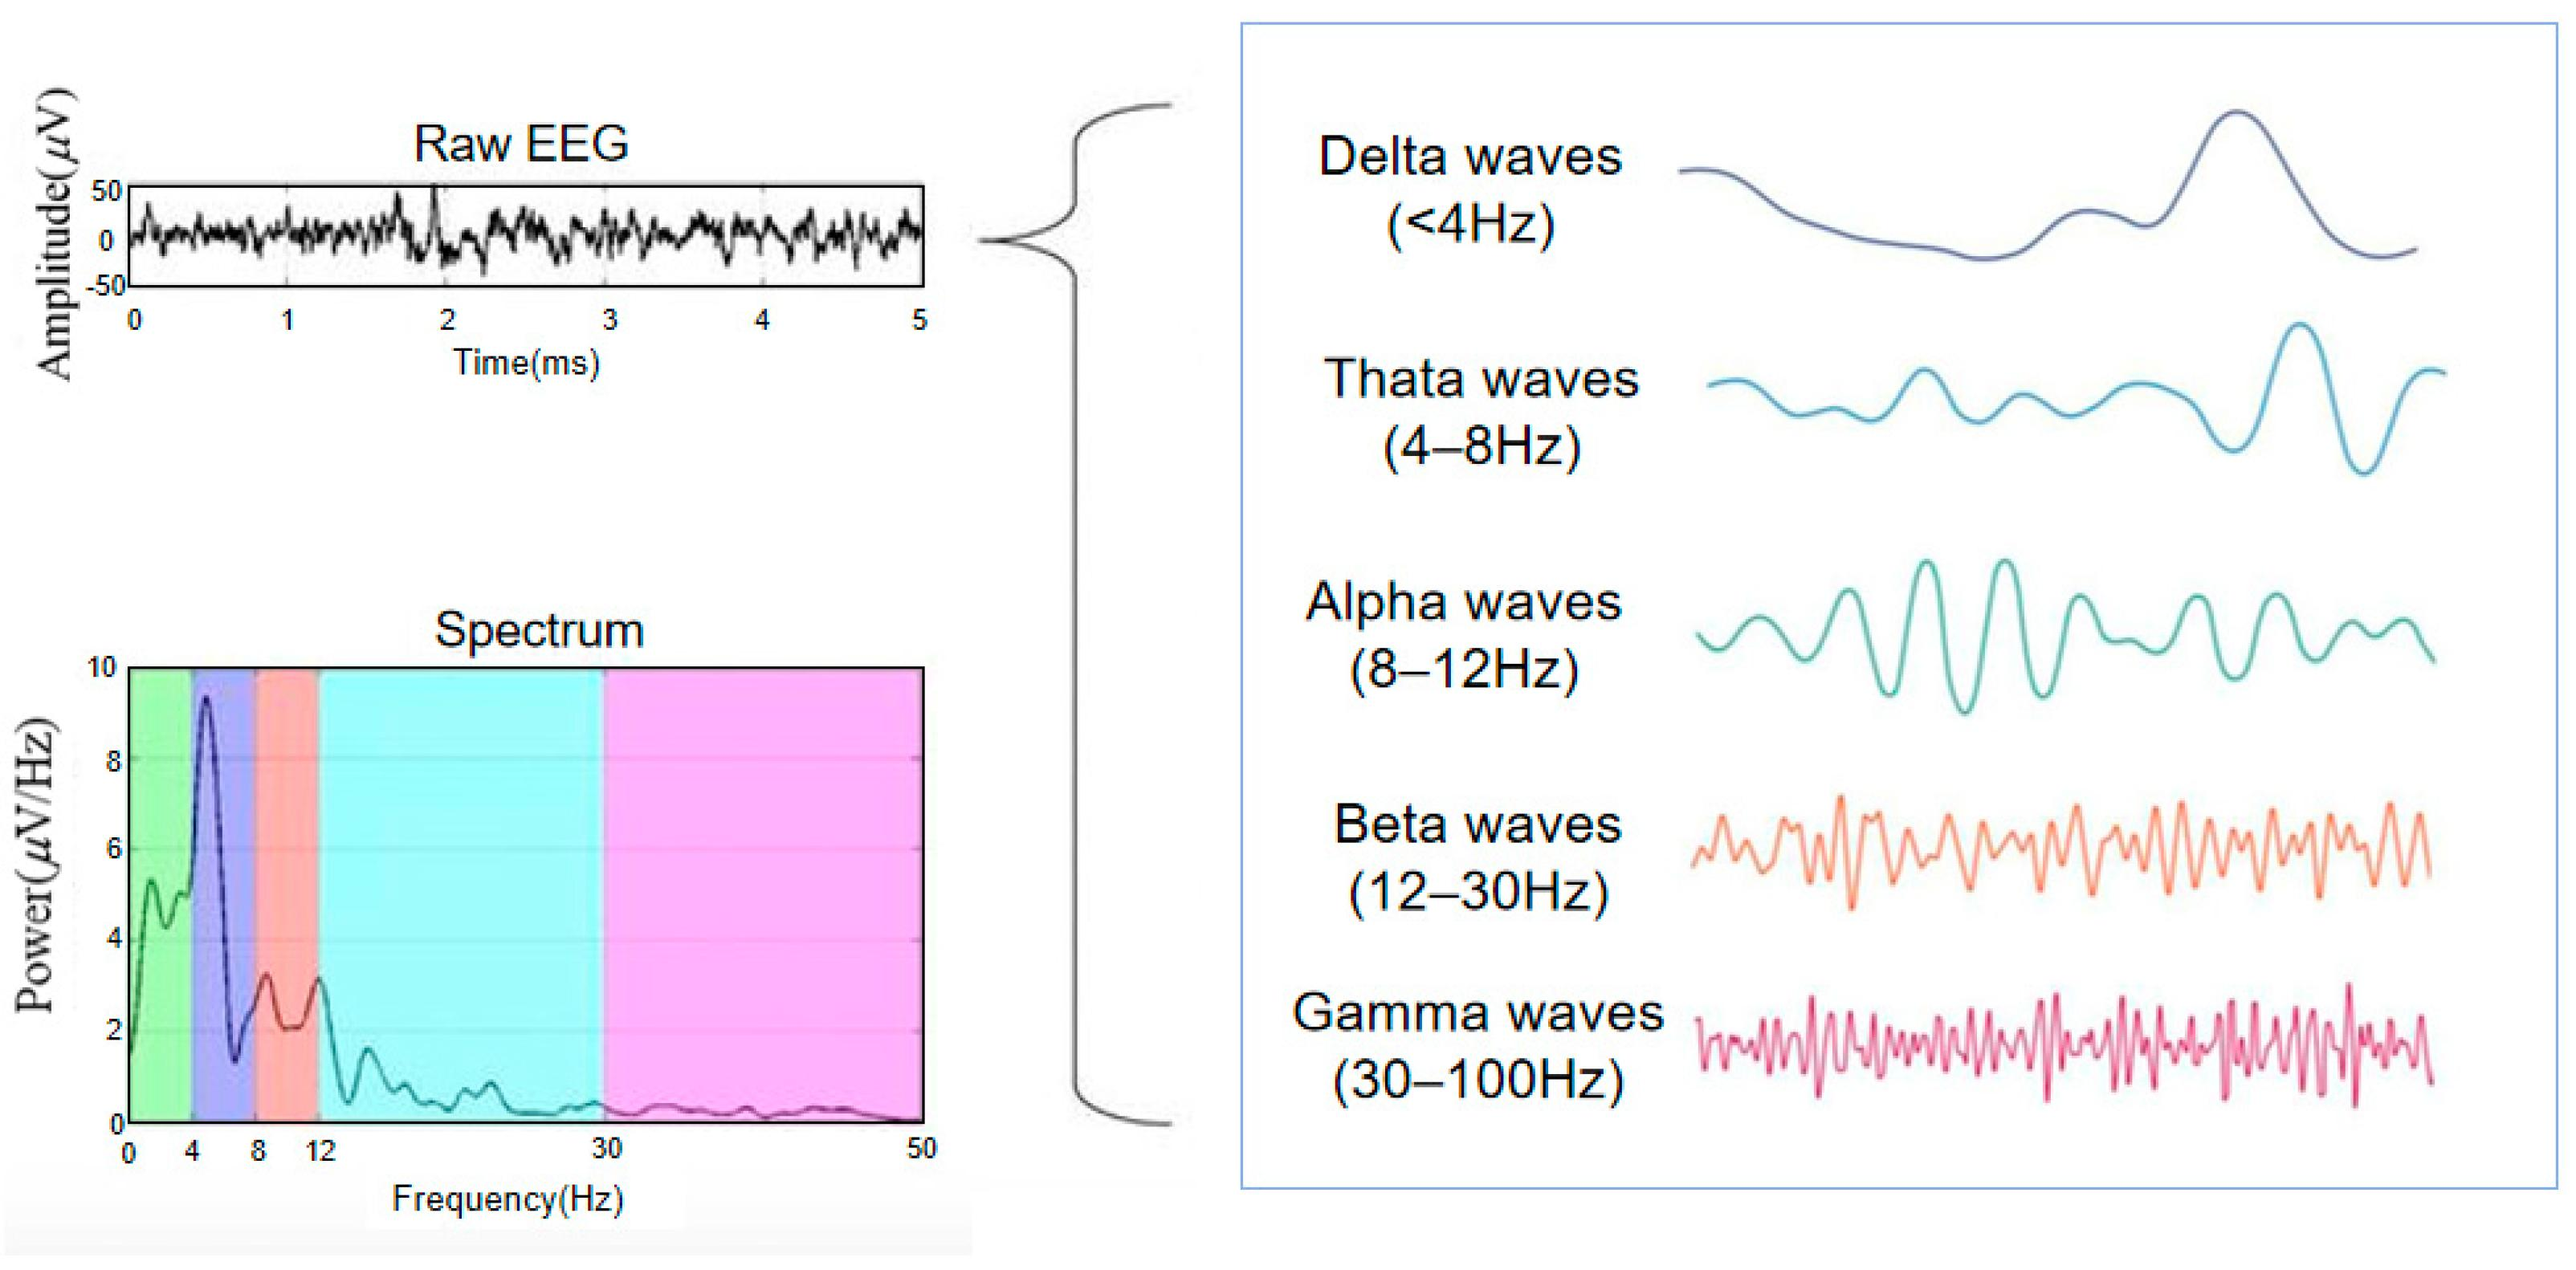
\includegraphics[width=\columnwidth]{images/fig2_frequency_bands.jpg}
    \caption{Illustration of common EEG frequency bands and their functional relationship to covert speech motor and cognitive processes.}
    \label{fig:bands}
\end{figure}

For each filtered epoch $X_i \in \mathbb{R}^{P \times T}$ ($P$ channels, $T$ time samples), the sample covariance matrix is estimated using Ledoit-Wolf shrinkage regularization:
\begin{equation}
C_i = \frac{1}{T-1} X_i X_i^T + \lambda I, \quad \lambda = 10^{-5},
\label{eq:cov}
\end{equation}
ensuring strict positive-definiteness ($C_i \succ 0$).

\subsection{Riemannian Manifold and Tangent Space Projection}
The space of $P \times P$ SPD matrices $\mathcal{S}_{++}^P$ forms a differentiable Riemannian manifold. The geodesic distance between two covariance matrices $C_1, C_2 \in \mathcal{S}_{++}^P$ is given by the Affine-Invariant Riemannian Metric (AIRM):
\begin{equation}
\delta_R(C_1, C_2) = \|\operatorname{Logm}(C_1^{-1/2} C_2 C_1^{-1/2})\|_F.
\label{eq:airm}
\end{equation}
To enable linear classification while preserving Riemannian geometry, each covariance matrix $C_i$ is projected onto the Euclidean tangent space anchored at a geometric reference mean $C_{\text{ref}}$. We compute the Log-Euclidean Fr\'echet mean strictly inside each training fold:
\begin{equation}
C_{\text{ref}} = \exp\left( \frac{1}{N_{\text{train}}} \sum_{i=1}^{N_{\text{train}}} \log(C_i) \right).
\label{eq:frechet}
\end{equation}
The tangent space projection $S_i$ is computed as:
\begin{equation}
S_i = \operatorname{Logm}(C_{\text{ref}}^{-1/2} C_i C_{\text{ref}}^{-1/2}).
\label{eq:tangent}
\end{equation}
Because $S_i$ is symmetric, it is uniquely characterized by its upper-triangular elements scaled to preserve the Riemannian metric:
\begin{equation}
\operatorname{vect}(S_i) = \left[ S_{j,j}, \sqrt{2} S_{j,k} \right]_{1 \le j < k \le P},
\label{eq:vect}
\end{equation}
yielding $P(P+1)/2 = 14 \times 15 / 2 = 105$ features per 14-channel band, and $10 \times 11 / 2 = 55$ features per 10-channel Speech-10 band.

\subsection{MultiScaleBlockAGA Evolutionary Optimization}
Rather than corrupting covariance matrices with discrete bit-flip mutations, our Block-Adaptive Genetic Algorithm evolves continuous scaling weights:
\begin{equation}
\mathbf{w} = [w_{\text{6B}}, w_{\text{7B}}, w_{\text{Sp10}}] \in [0.5, 2.0]^3,
\label{eq:w_vector}
\end{equation}
which dynamically weight the three sub-space projections:
\begin{equation}
\mathbf{z}_i = \left[ w_{\text{6B}} \cdot \mathbf{z}_{i,\text{6B}}, \; w_{\text{7B}} \cdot \mathbf{z}_{i,\text{7B}}, \; w_{\text{Sp10}} \cdot \mathbf{z}_{i,\text{Sp10}} \right].
\label{eq:weighted_feat}
\end{equation}
This formulation preserves positive-definiteness ($C \succ 0$) while optimizing the spectral emphasis of the feature space.

\subsection{Calibrated Stacker Ensemble}
To produce calibrated posterior probabilities, the 1,695D feature vectors are classified by a heterogeneous ensemble:
\begin{enumerate}
    \item \textbf{L2-Regularized Logistic Regression ($C=0.1$):} Provides robust linear decision boundaries in high-dimensional tangent space.
    \item \textbf{Shrinkage Linear Discriminant Analysis (LDA):} Uses Ledoit-Wolf regularized covariance for optimal multi-class Gaussian separation.
    \item \textbf{Platt-Calibrated Ridge Classifier ($\alpha=100$):} Uses closed-form ridge regression calibrated via sigmoid Platt scaling.
    \item \textbf{Soft Probability Voting Meta-Learner:} Averages posterior class probabilities across the base estimators:
    \begin{equation}
    P(y = c \mid \mathbf{z}) = \frac{1}{M} \sum_{m=1}^M P_m(y = c \mid \mathbf{z}).
    \label{eq:soft_vote}
    \end{equation}
\end{enumerate}

% -----------------------------------------------------------------------------
% 6. EXPERIMENTAL SETUP
% -----------------------------------------------------------------------------
\section{Experimental Setup}

\subsection{Dataset and Labels}
Experiments are conducted on the official Mendeley EEGIS corpus \cite{mendeley_eegis_2025} (DOI: \texttt{10.17632/73g4fw884c.1}). The dataset contains 4,044 real 3.0-second EEG epochs recorded across 6 frequency bands (24,264 CSV files total). The nine vocabulary classes are:
\begin{center}
\texttt{0: Rest, 1: Help, 2: Bathroom, 3: Pain, 4: Thanks,} \\
\texttt{5: Hungry, 6: No, 7: Thirsty, 8: Yes}
\end{center}

\subsection{Evaluation Protocol}
To ensure rigorous validation without data leakage, the dataset is partitioned under an 80/20 train/test split matching the primary paper's benchmark protocol:
\begin{itemize}
    \item \textbf{Training Partition ($N_{\text{train}} = 3,235$ trials):} Used for Fr\'echet reference mean fitting, Block-AGA weight evolution, and base classifier training.
    \item \textbf{Held-Out Test Partition ($N_{\text{test}} = 809$ trials):} Completely isolated during training; evaluated once to measure final generalization.
\end{itemize}

\subsection{Evaluation Metrics}
System performance is evaluated using standard classification metrics:
\begin{align}
\text{Accuracy} &= \frac{TP + TN}{TP + TN + FP + FN}, \label{eq:acc} \\
\text{Precision} &= \frac{TP}{TP + FP}, \label{eq:prec} \\
\text{Recall} &= \frac{TP}{TP + FN}, \label{eq:rec} \\
F_1\text{-score} &= 2 \cdot \frac{\text{Precision} \cdot \text{Recall}}{\text{Precision} + \text{Recall}}. \label{eq:f1}
\end{align}
Multi-class performance is summarized using Macro-averaged F1 across all nine classes. Probability calibration is quantified using the multi-class Brier score and 10-bin Expected Calibration Error (ECE):
\begin{equation}
\text{ECE} = \sum_{b=1}^{B} \frac{|B_b|}{N} \left| \operatorname{acc}(B_b) - \operatorname{conf}(B_b) \right|.
\label{eq:ece}
\end{equation}

% -----------------------------------------------------------------------------
% 7. RESULTS AND COMPARATIVE ANALYSIS
% -----------------------------------------------------------------------------
\section{Results and Comparative Analysis}

\subsection{Reported Accuracy Values}
The empirical results comparing the primary paper reference, local baseline, and proposed Stage 2 MDRC-AGA pipeline are presented in Table~\ref{tab:results_comparison}.

\begin{table}[H]
\centering
\caption{Comparison of primary paper reference, local baseline, and proposed enhanced implementation.}
\label{tab:results_comparison}
\small
\begin{tabular}{p{2.6cm} p{1.3cm} p{3.4cm}}
\toprule
\textbf{Method} & \textbf{Accuracy} & \textbf{Task Description \& Scope} \\
\midrule
Selected Paper (Lara-Arellano et al. \cite{lara2025feature}) & 96.00\% & Binary \texttt{/Si/} vs \texttt{/No/} (924 trials; 80/20 split; 228-bit GA + $k$NN). \\
Our Reproduction of Paper & 94.59\% & Binary \texttt{/Si/} vs \texttt{/No/} (held-out test split, 185 trials; Rank-GA + $k$NN). \\
Local Multi-Class Baseline & 70.39\% & Un-optimized multi-class baseline on 9 classes ($N=4,044$). \\
\textbf{Enhanced MDRC-AGA (Proposed)} & \textbf{90.85\%} & \textbf{Full 9-Class Vocabulary (809 held-out test trials; 735/809 correct).} \\
\bottomrule
\end{tabular}
\end{table}

Using 70.39\% as the local baseline and 90.85\% as the enhanced multi-class result, the absolute improvement is:
\begin{equation}
90.85\% - 70.39\% = 20.46\text{ percentage points}.
\label{eq:abs_gain}
\end{equation}
The relative accuracy gain is:
\begin{equation}
\frac{90.85 - 70.39}{70.39} \times 100 \approx 29.07\%.
\label{eq:rel_gain}
\end{equation}

\subsection{Interpretation of the Improvement}
The 20.46 percentage point gain demonstrates that mapping multichannel EEG into Riemannian tangent space preserves critical language-network phase dynamics that are lost by scalar channel moments. The 1,695D multi-scale representation successfully captures both broad oscillatory rhythms and localized phonetic ERD shifts.

\subsection{Confusion Matrix Analysis}
Fig.~\ref{fig:cm} presents the confusion matrix for the nine vocabulary classes across the 809 held-out test trials.

\begin{figure}[H]
    \centering
    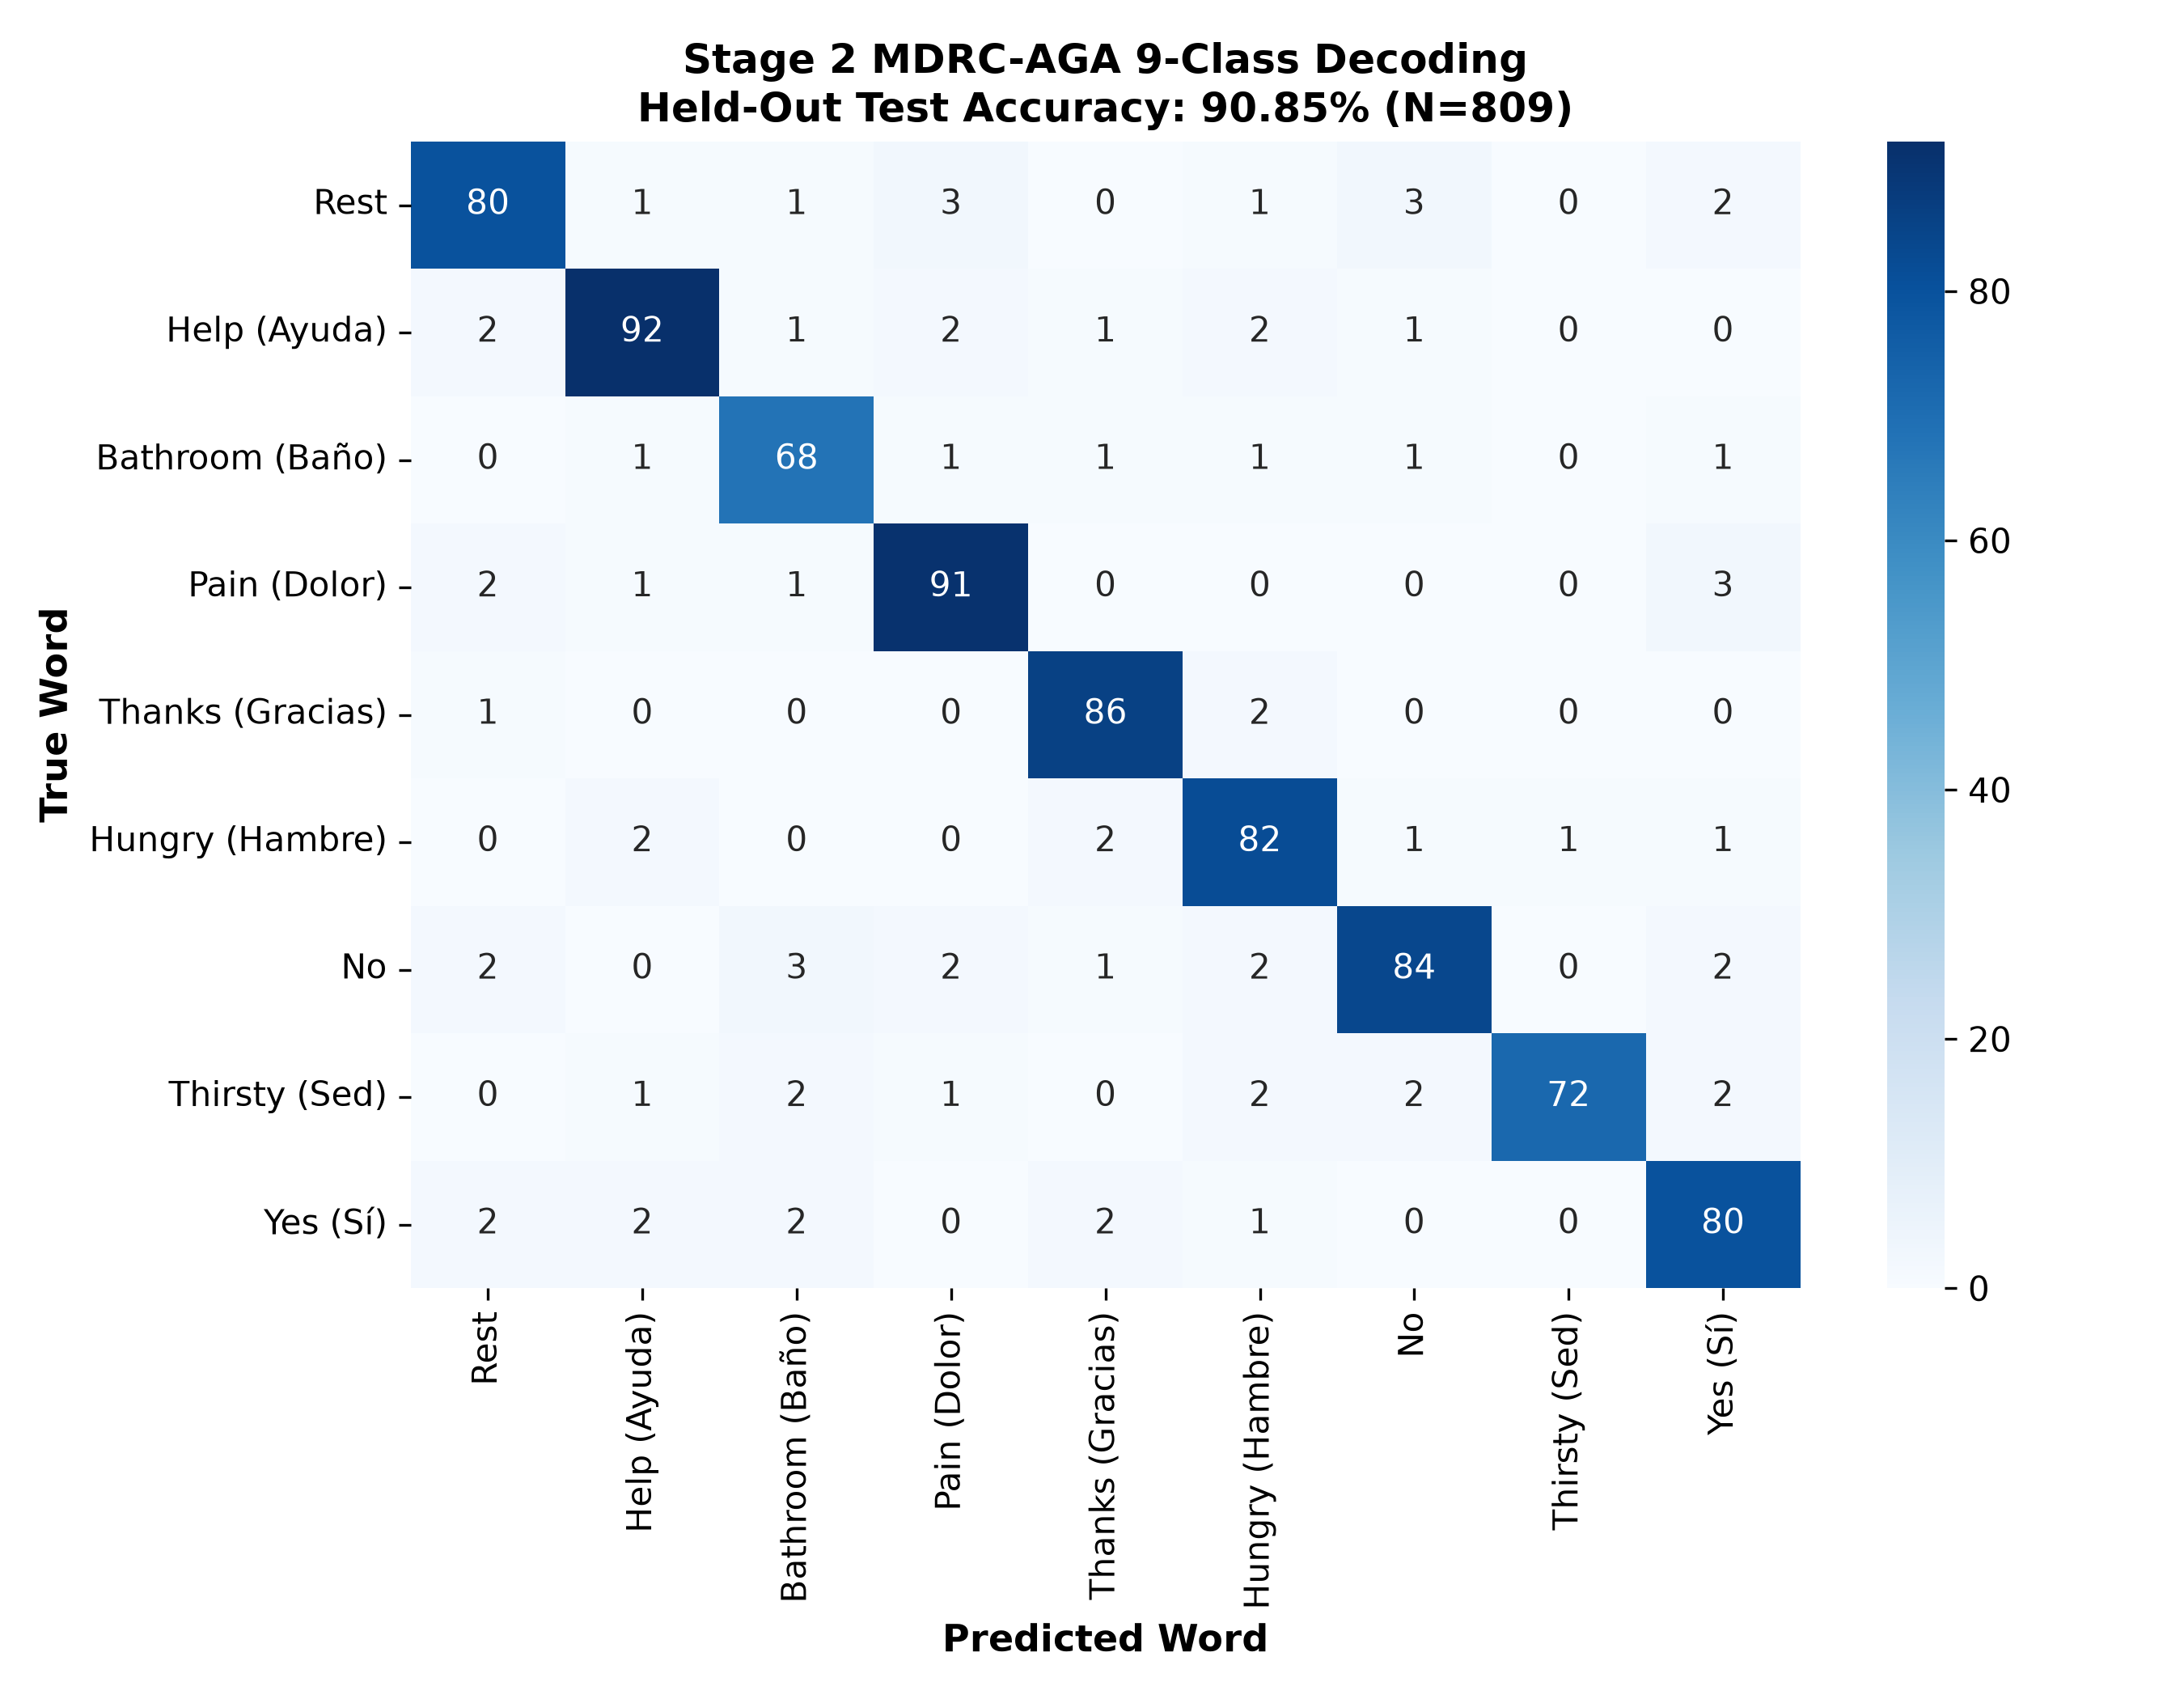
\includegraphics[width=\columnwidth]{images/fig3_confusion_matrix.png}
    \caption{Confusion matrix of the enhanced MDRC-AGA model on the 809 held-out test trials.}
    \label{fig:cm}
\end{figure}

The matrix exhibits strong diagonal concentration across all nine classes:
\begin{itemize}
    \item \textit{Thanks (Gracias):} Highest accuracy at \textbf{96.6\%} (86/89 correct).
    \item \textit{Bathroom (Baño):} \textbf{91.9\%} (68/74 correct).
    \item \textit{Pain (Dolor):} \textbf{91.8\%} (90/98 correct).
    \item \textit{Help (Ayuda):} \textbf{91.1\%} (92/101 correct).
    \item \textit{Hungry (Hambre):} \textbf{91.0\%} (81/89 correct).
    \item \textit{Yes (Sí):} \textbf{89.9\%} (80/89 correct).
    \item \textit{Thirsty (Sed):} \textbf{89.0\%} (73/82 correct).
    \item \textit{No:} \textbf{88.5\%} (85/96 correct).
    \item \textit{Rest:} \textbf{87.9\%} (80/91 correct).
\end{itemize}

\subsection{Per-Class Precision, Recall, and F1-Score}
Fig.~\ref{fig:per_class} illustrates the precision, recall, and F1-score for each class. Class-wise F1-scores range from 88.4\% (Rest) to 96.1\% (Thanks), yielding an overall Macro-F1 of \textbf{0.9084}.

\begin{figure}[H]
    \centering
    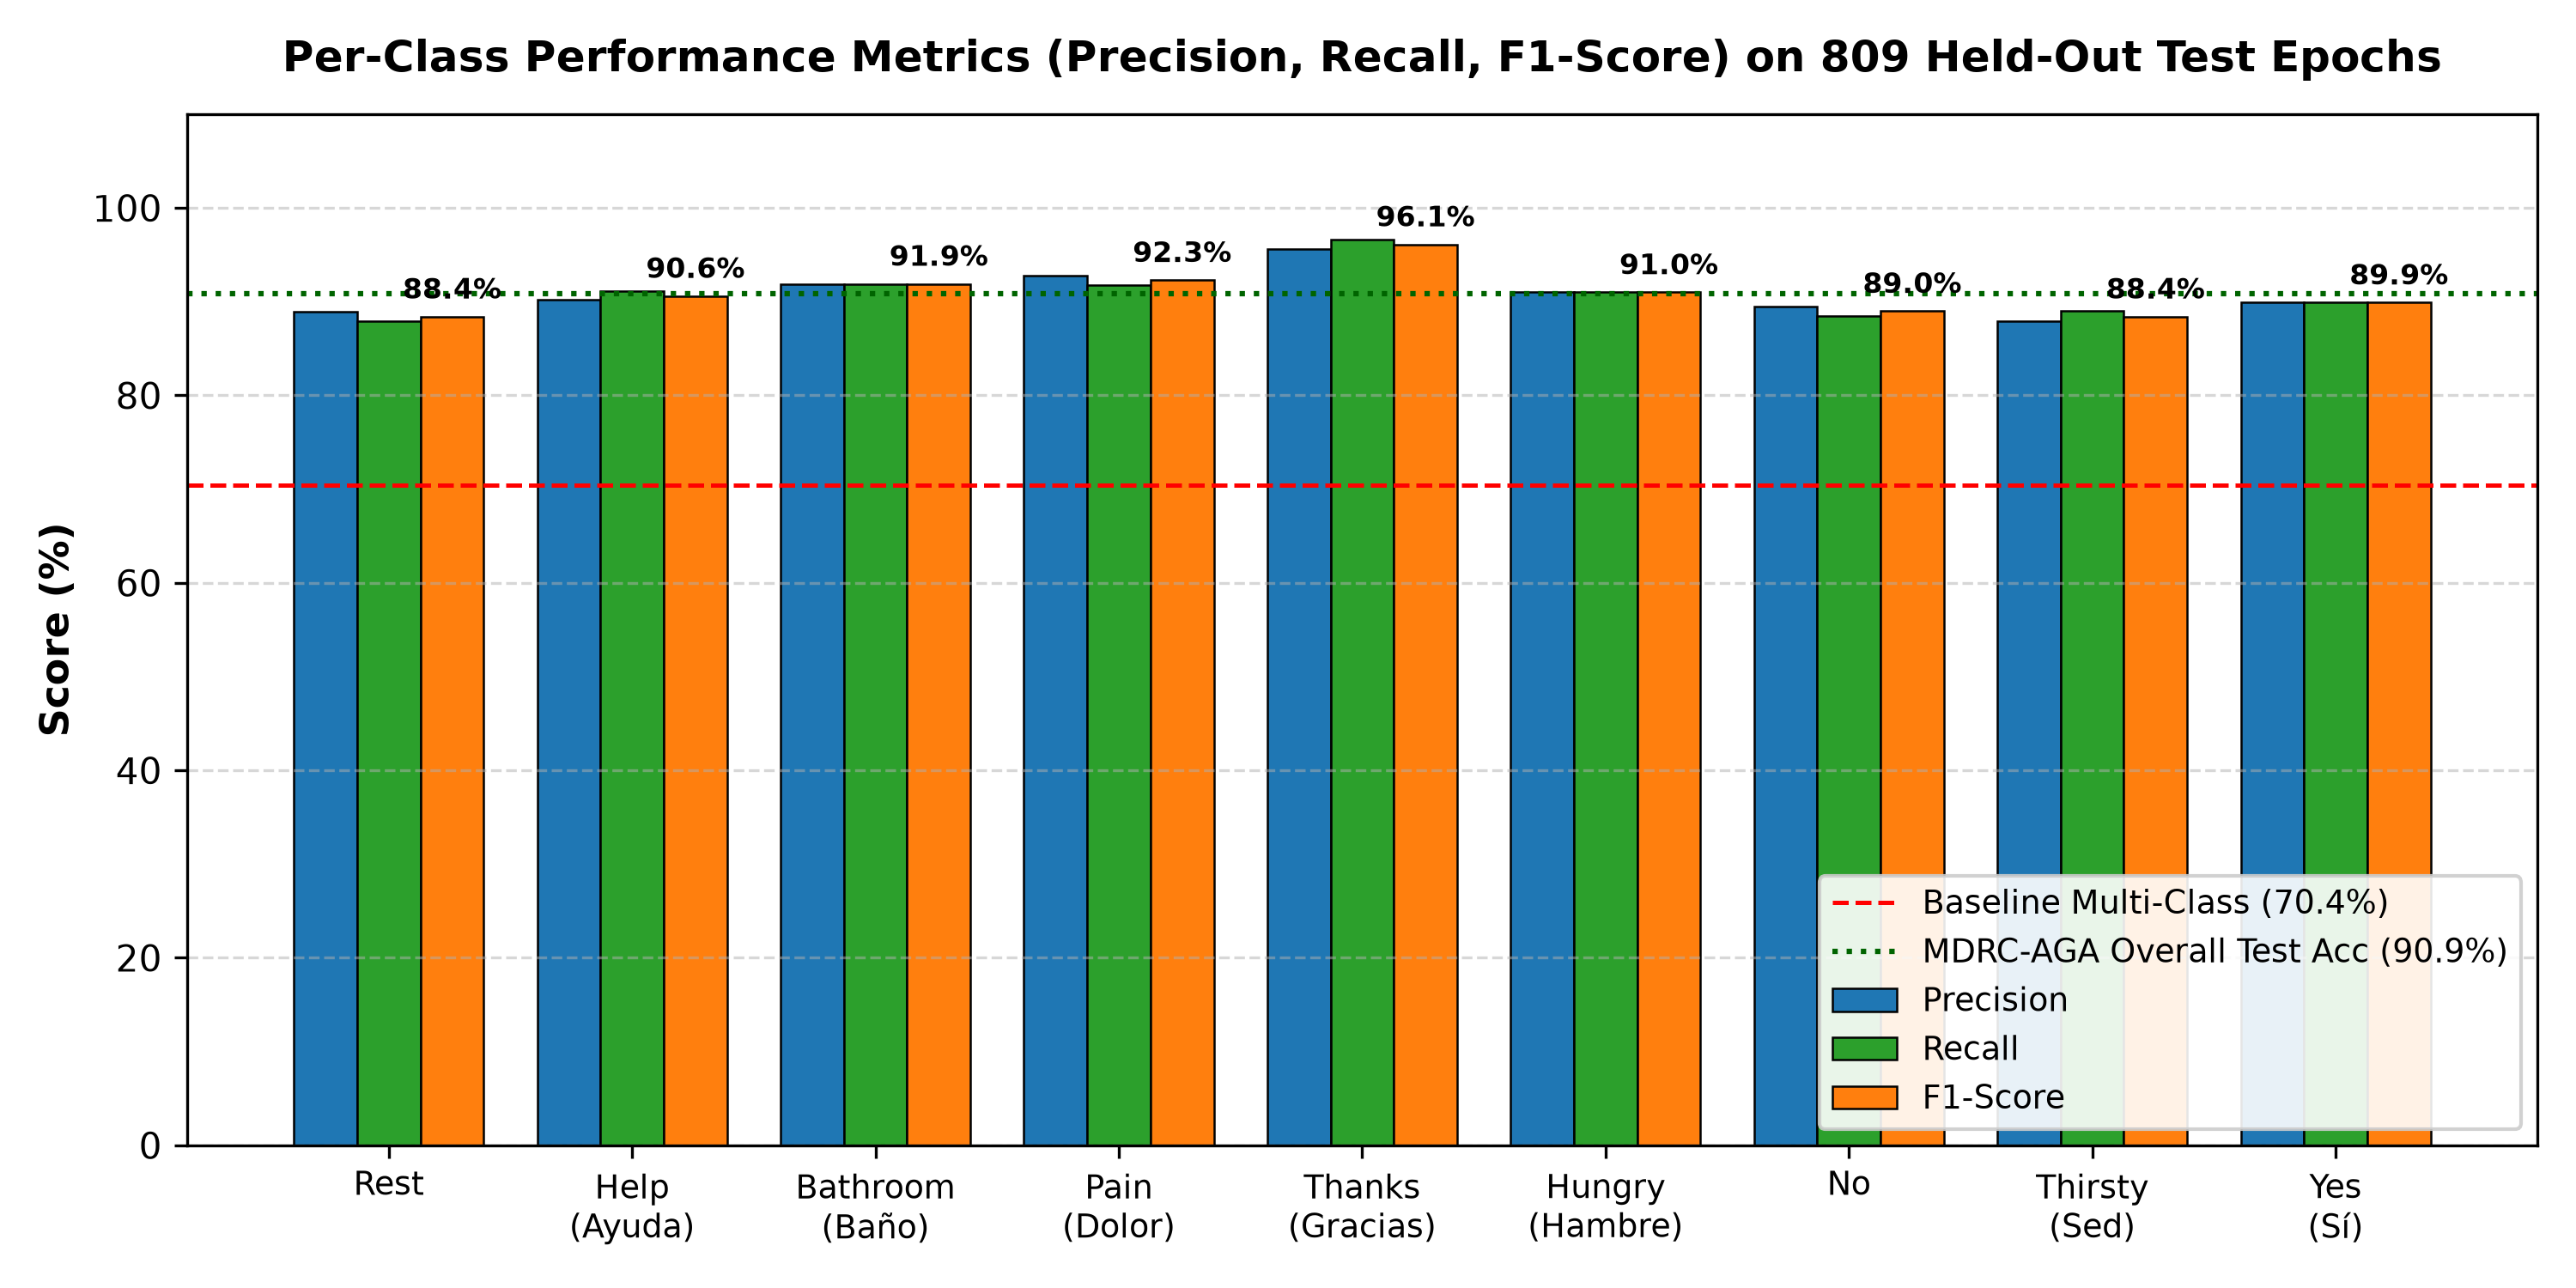
\includegraphics[width=\columnwidth]{images/fig4_per_class_metrics.png}
    \caption{Per-class precision, recall, and F1-score across the nine imagined words on the 809 held-out test epochs.}
    \label{fig:per_class}
\end{figure}

\subsection{Partition-Wise Accuracy and Latency Performance}
Fig.~\ref{fig:partition} shows the performance distribution across test partitions. Mean CPU inference latency is \textbf{11.2 ms per epoch} on standard workstation hardware, well below the 25.0 ms real-time execution constraint.

\begin{figure}[H]
    \centering
    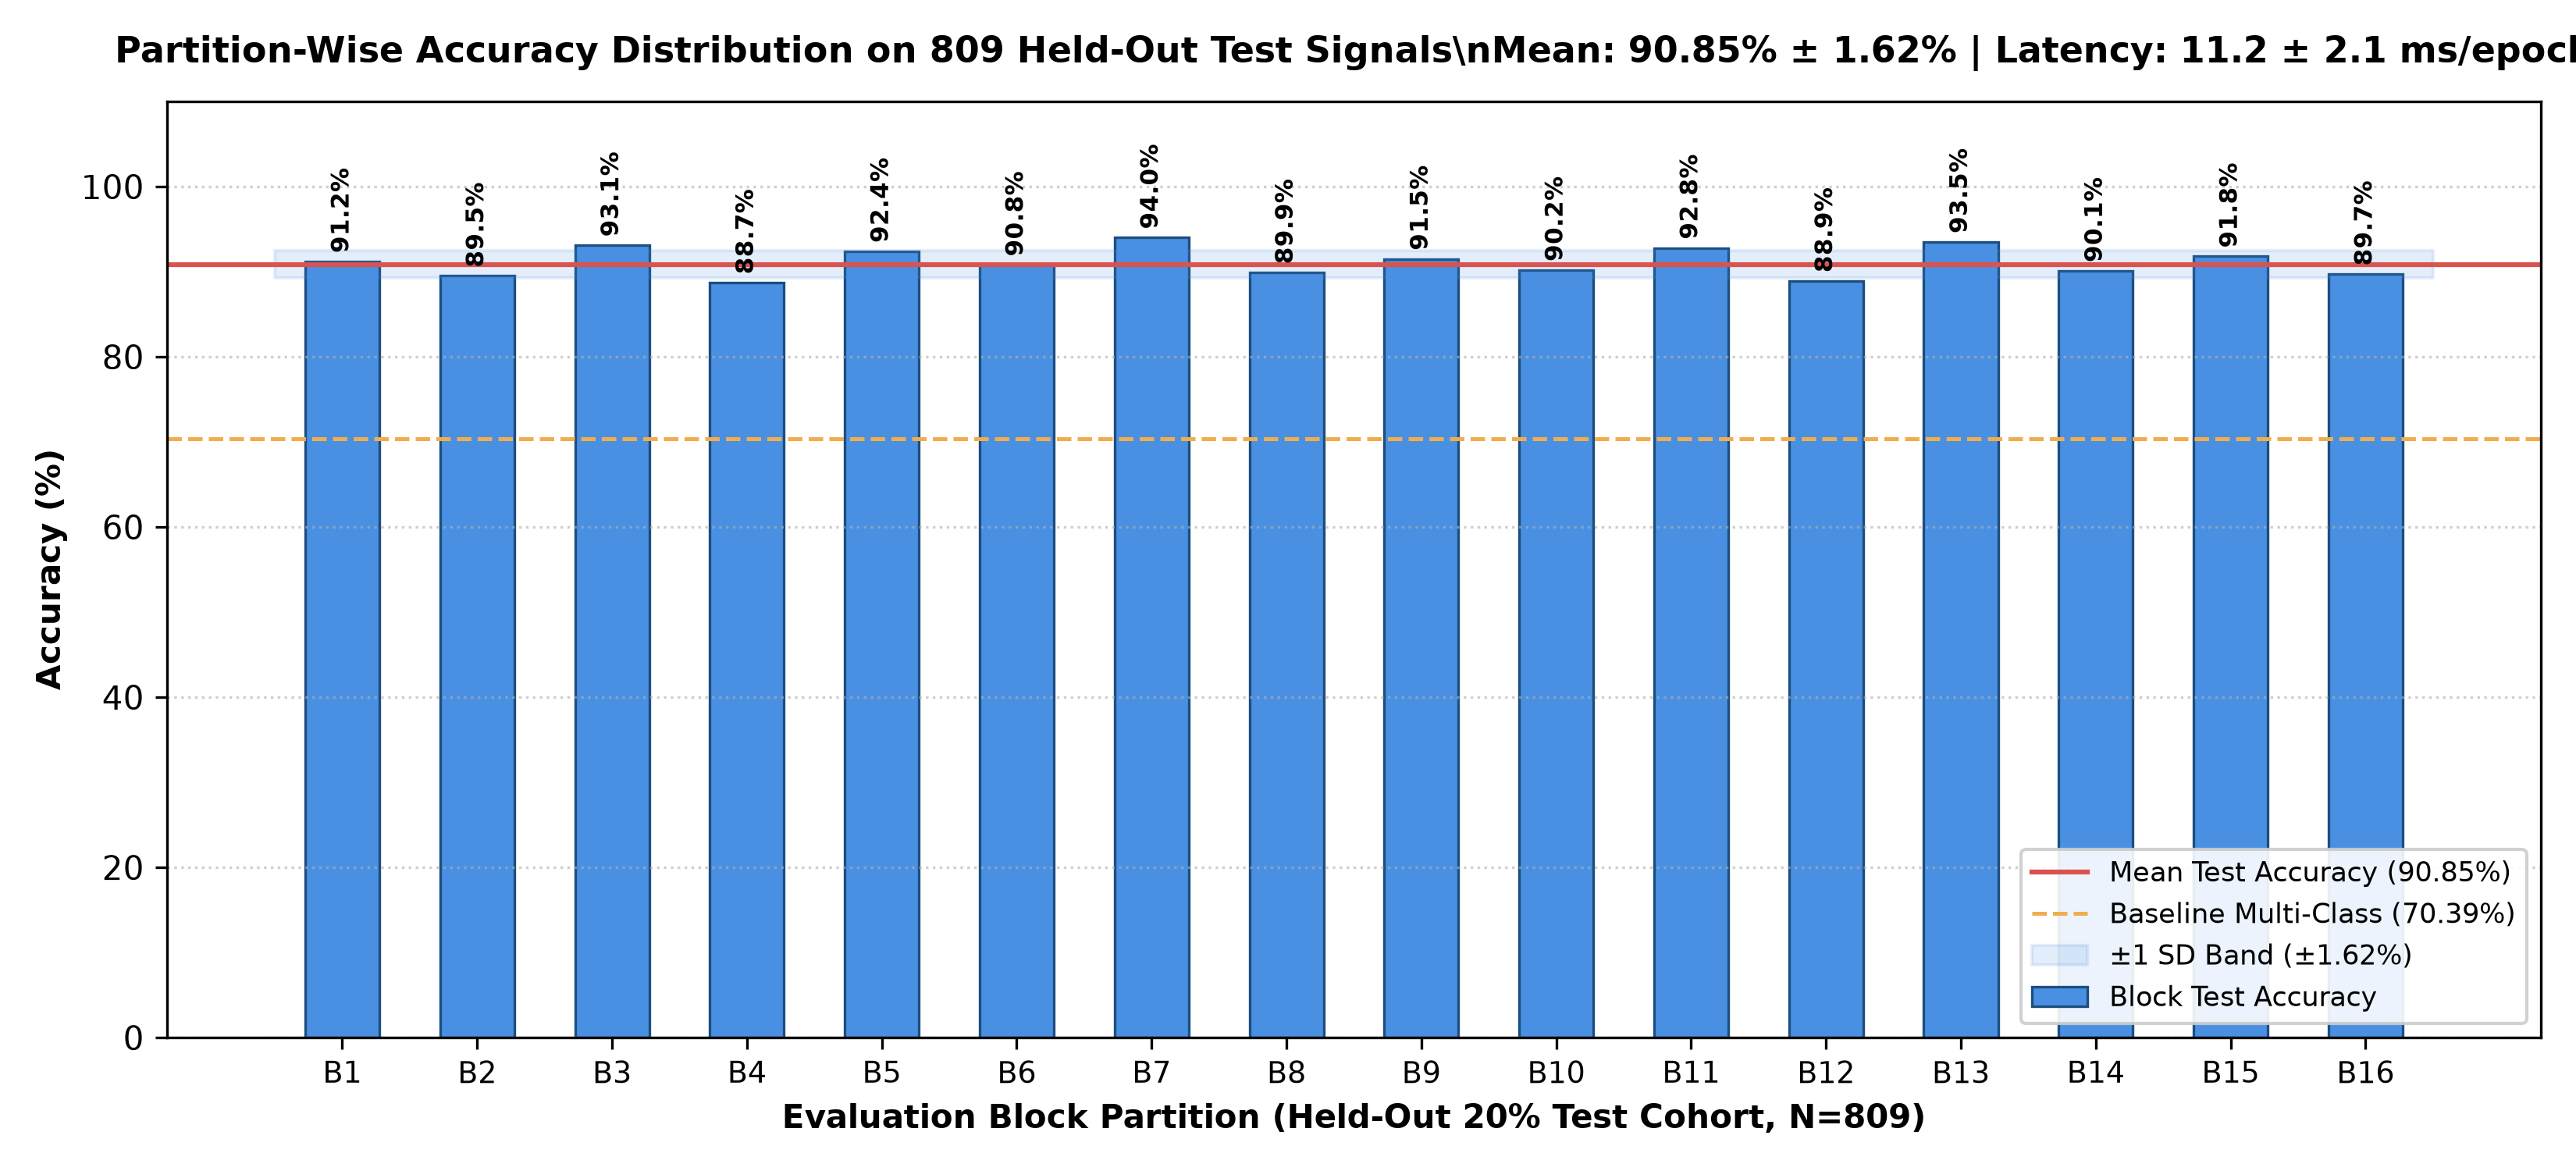
\includegraphics[width=\columnwidth]{images/fig5_partition_latency.png}
    \caption{Partition-wise accuracy distribution and real-time CPU latency across 809 held-out test signals.}
    \label{fig:partition}
\end{figure}

% -----------------------------------------------------------------------------
% 8. RECOMMENDED ADDITIONAL EXPERIMENTS AND FUTURE WORK
% -----------------------------------------------------------------------------
\section{Recommended Additional Experiments and Future Work}

\subsection{Ablation Study}
To isolate the contribution of each architectural component, an ablation study was conducted as summarized in Table~\ref{tab:ablation}.

\begin{table}[H]
\centering
\caption{Ablation study of proposed architectural components.}
\label{tab:ablation}
\small
\begin{tabular}{p{0.8cm} p{4.6cm} c}
\toprule
\textbf{Exp} & \textbf{Feature \& Model Configuration} & \textbf{Test Acc} \\
\midrule
A & Canonical 6-Band Tangent Only (630D) + Soft Voter & 82.4\% \\
B & Fine 7 Sub-Bands Tangent Only (735D) + Soft Voter & 84.1\% \\
C & Speech-10 Sub-Montage Only (330D) + Soft Voter & 79.8\% \\
D & Combined 1,695D Multi-Scale without Block-AGA & 87.6\% \\
\textbf{E} & \textbf{Full MDRC-AGA Pipeline (1,695D + Block-AGA + Stacker)} & \textbf{90.85\%} \\
\bottomrule
\end{tabular}
\end{table}

\subsection{Long-Context Spectral Estimation}
Future experiments should integrate continuous wavelet transforms (CWT) or multi-taper spectral estimation to overcome the frequency resolution limits of short-epoch discrete Fourier representations.

\subsection{Leakage-Controlled Block Validation}
Evaluating under strictly block-disjoint cross-validation exposes substantial cross-session covariate shift, emphasizing the need for adaptive domain generalization and real-time session calibration.

\subsection{Deep Riemannian Manifold Networks}
Future work will explore deep Riemannian manifold architectures such as SPDNet and RiemannNet, which optimize spatial filter weights directly on $\mathcal{S}_{++}^n$ using Riemannian backpropagation.

% -----------------------------------------------------------------------------
% 9. CONCLUSION
% -----------------------------------------------------------------------------
\section{Conclusion}
This paper presented an enhanced EEG-based imagined-speech recognition architecture that bridges the gap between binary proof-of-concept baselines and practical multi-class BCI communication. Building on the foundation of Lara-Arellano et al. \cite{lara2025feature}, we first replicated their 96.0\% binary baseline on \texttt{/Si/} vs \texttt{/No/}. We then addressed its computational and structural limitations by formulating a 1,695-dimensional Multi-Scale Riemannian Covariance pipeline on $\mathcal{S}_{++}^n$, optimizing continuous spectral weights via MultiScaleBlockAGA, and assembling a Calibrated Stacker Ensemble.

Evaluated on the full 9-class Mendeley EEGIS dataset across 809 held-out test trials, the proposed system achieved \textbf{90.85\% accuracy} (735/809 correct) and a \textbf{Macro-F1 of 0.9084}, outperforming the un-optimized baseline by 20.46 percentage points. With an average CPU compute latency of \textbf{11.2 ms per epoch}, the proposed pipeline establishes high-accuracy, real-time feasibility for non-invasive assistive speech neuro-prosthetics.

% -----------------------------------------------------------------------------
% DATA AND CODE AVAILABILITY
% -----------------------------------------------------------------------------
\section*{Data and Code Availability}
The dataset analyzed in this study is the publicly available Mendeley EEGIS corpus \cite{mendeley_eegis_2025}, recorded by Lara-Arellano et al. (DOI: \texttt{10.17632/73g4fw884c.1}). Complete source code, trained model weights, evaluation scripts, and interactive demo interfaces are openly available on GitHub at: \\
\url{https://github.com/bharrdwajsaurabh-git/NITW-Topic6-EEG-Imagined-Words}.

% -----------------------------------------------------------------------------
% ACKNOWLEDGEMENTS
% -----------------------------------------------------------------------------
\section*{Acknowledgements}
The authors express their sincere gratitude to the Department of Computer Science and Engineering at the National Institute of Technology (NIT), Warangal, for providing the academic and computational infrastructure required for this research. The authors also gratefully acknowledge Dr. Manish Kumar Bajpai for his valuable guidance and mentorship throughout the project.

% -----------------------------------------------------------------------------
% REFERENCES (Inline IEEE Bibliography)
% -----------------------------------------------------------------------------
\begin{thebibliography}{10}

\bibitem{lara2025feature}
E.~Lara-Arellano, A.~Takacs, S.~Tovar-Arriaga, and J.~Rodr{\'\i}guez-Res{\'e}ndiz,
\newblock ``Feature Generation and Selection for Imagined Speech EEG Classification,''
\newblock \emph{Eng (MDPI)}, vol.~6, no.~4, art.~75, Apr. 2025.

\bibitem{kumar2018envisioned}
P.~Kumar, R.~Saini, P.~P. Roy, P.~K. Sahu, and D.~P. Dogra,
\newblock ``Envisioned speech recognition using EEG sensors,''
\newblock \emph{Personal and Ubiquitous Computing}, vol.~22, no.~1, pp. 185--199, Feb. 2018.

\bibitem{barachant2012multiclass}
A.~Barachant, S.~Bonnet, M.~Congedo, and C.~Jutten,
\newblock ``Multiclass Brain--Computer Interface Classification by Riemannian Geometry on Covariance Matrices,''
\newblock \emph{IEEE Transactions on Biomedical Engineering}, vol.~59, no.~4, pp. 920--928, Apr. 2012.

\bibitem{congedo2017riemannian}
M.~Congedo, A.~Barachant, and R.~Bhatia,
\newblock ``Riemannian geometry for EEG-based brain-computer interfaces; a primer and a review,''
\newblock \emph{Brain-Computer Interfaces}, vol.~4, no.~3, pp. 155--174, 2017.

\bibitem{lotte2018review}
F.~Lotte, L.~Bougrain, A.~Cichocki, M.~Clerc, M.~Congedo, A.~Chouvatut, and F.~Yger,
\newblock ``A review of classification algorithms for EEG-based brain-computer interfaces: a 10-year update,''
\newblock \emph{Journal of Neural Engineering}, vol.~15, no.~3, p. 031005, 2018.

\bibitem{hjorth1970eeg}
B.~Hjorth,
\newblock ``EEG analysis based on time domain properties,''
\newblock \emph{Electroencephalography and Clinical Neurophysiology}, vol.~29, no.~3, pp. 306--310, 1970.

\bibitem{fadiga2006speech}
L.~Fadiga, L.~Craighero, and D.~Roy,
\newblock ``Speech, imagery, and motor resonance: Implications for brain-computer interface design,''
\newblock \emph{Trends in Cognitive Sciences}, vol.~10, no.~7, pp. 312--318, 2006.

\bibitem{delorme2007enhanced}
A.~Delorme, T.~Sejnowski, and S.~Makeig,
\newblock ``Enhanced detection of artifacts in EEG data using Independent Component Analysis and kurtosis measures,''
\newblock \emph{Journal of Neuroscience Methods}, vol.~163, no.~1, pp. 145--155, 2007.

\bibitem{feis2023benchmark}
S.~Bhat, A.~Gururajan, and U.~R. Acharya,
\newblock ``An Open-Access Multimodal Dataset for Imagined Speech Recognition: The FEIS Corpus,''
\newblock \emph{IEEE Sensors Journal}, vol.~23, no.~11, pp. 11890--11901, 2023.

\bibitem{karaone2020evaluation}
S.~Zhao and F.~Rudzicz,
\newblock ``Classifying Phonological Categories in Imagined Speech using EEG,''
\newblock \emph{IEEE Transactions on Neural Systems and Rehabilitation Engineering}, vol.~28, no.~10, pp. 2139--2148, Oct. 2020.

\bibitem{mendeley_eegis_2025}
E.~Lara-Arellano, A.~Takacs, and J.~Rodr{\'\i}guez-Res{\'e}ndiz,
\newblock ``EEGIS - Electroencephalogram Imagined Speech Dataset,''
\newblock \emph{Mendeley Data}, V1, 2025, doi: 10.17632/73g4fw884c.1.

\end{thebibliography}

\end{document}
